\documentclass[paper=a4,nenglish]{scrartcl}
%\usepackage[T1]{fontenc}
\usepackage[utf8]{inputenc}
\usepackage{a4wide}
\setcounter{secnumdepth}{3}
\setcounter{tocdepth}{3}
\setlength\parskip{\medskipamount}
\setlength\parindent{0pt}
\usepackage{float}
\usepackage{makeidx}
\usepackage{listings}																
%\usepackage{babel}
\usepackage{setspace}
\usepackage{epsfig}
\usepackage{multirow}
\usepackage{color}
\usepackage{textcomp}

\usepackage[
  pdftex, 
  colorlinks=true,
  linkcolor=blue,
  urlcolor=blue,
  citecolor=blue,  		
  linkcolor=black,
  urlcolor=black,
  citecolor=black,
  plainpages=false,
  pdfpagelabels,
	pdftitle={Bla},
	pdfauthor={Michael Frey}
]{hyperref}

% Definition fuer Farbschema Rot (RGB: 193, 24, 24)
\definecolor{defred}{rgb}{0.75,0.09,0.09}
% Definition fuer Farbschema Gruen (RGB: 193, 24, 24)
\definecolor{defgreen}{rgb}{0.43,0.68,0.18}
% Definition fuer Farbschema Blau (RGB: 41, 104, 208)
\definecolor{defblue}{rgb}{0.16,0.4,0.81}
% Definition fuer Farbschema Orange (RGB: 255, 139, 0)
\definecolor{deforange}{rgb}{1,0.54,0}


\lstloadlanguages{Java}
\lstset{
  language=[AspectJ]Java,						% Java with AspectJ-Dialect
	tabsize=2,												% Tabulatorbreite
	linewidth=\linewidth,							% Width of a line
	breaklines=true,									% Break long lines
	breakatwhitespace=true,						% Only break at whitespaces
	basicstyle=\scriptsize\ttfamily,	% Schriftart/-größe	
	numbers=left,											% Linenumbers left
	numberfirstline=false,						% Not: Always number 1. line
	numberstyle=\scriptsize,					% Größe der Zeilennummern
	stepnumber=2,											% Jede 2. Zeilennummer anzeigen
	numbersep=5pt,										% Abstand Nr - Quellcode
	showspaces=false,									% Spaces nicht anzeigen
	showtabs=false,										% Tabs nicht anzeigen
	showstringspaces=false,						% Don't show tabs in strings
	showlines=false,									% Leerzeilen am Sourceende weglassen
	extendedchars=true,								% ASCII-Zeichnen > 127 zulassen 
	identifierstyle=\textbf,					% Identifier
	keywordstyle=\bfseries,						% Keywords
	commentstyle=\itshape,						% Style of comments
	stringstyle=\ttfamily,						% Strings (!= Keywords)
	flexiblecolumns=false,						% Use fixed width for fonts
	fontadjust=true,									% "Base width" nicht jede Zeile anpassen
	frame=trbl,												% Frame; trBL
	captionpos=b,											% Position of the caption
	aboveskip=25pt,										% Space between text and the top of the listing
}


\lstdefinelanguage{Flow}{
  morekeywords={structure, stream, processing, datatype, package, using, namespace, use, tag, join, ejoin, map, std, avg, in, out, untag,
  count, int, float, string, boolean, now, last, elements, min, hrs, sec, match, split, import, if, else, return, operator, filter,
  diff, sdif, swrl, ocl, add, sub, div, mult, mod},
  sensitive=false,
  morecomment=[l]{//},
  morecomment=[s]{/*}{*/},
  morestring=[b]",
  keywordstyle=\bfseries\color{defblue},
  commentstyle=\bfseries\color{defgreen},
  stringstyle=\bfseries\color{defgreen},
  identifierstyle=\bfseries\color{deforange},
  basicstyle=\scriptsize\ttfamily,	
  showstringspaces=false,
  numberstyle=\scriptsize,					
  captionpos=b,
  tabsize=4,
  stepnumber=1,										
  breaklines=true
}

\lstdefinelanguage{Lua}{
  morekeywords={fm, create_operator_of_type, set_parameter, connect_operators},
  sensitive=false,
  morecomment=[l]{--},
  morecomment=[s]{--[[}{--]]},
  morestring=[b]",
  keywordstyle=\bfseries\color{defblue},
  commentstyle=\bfseries\color{defred},
  stringstyle=\bfseries\color{defgreen},
  identifierstyle=\bfseries\color{deforange},
  basicstyle=\scriptsize\ttfamily,	
  showstringspaces=false,
  numberstyle=\scriptsize,					
  captionpos=b,
  tabsize=4,
  stepnumber=1,										
  breaklines=true
}


\lstdefinelanguage{CMD}{
  morekeywords={mvn, package, Dtycho, javadoc, targetPlatform, test},
  sensitive=false,
  morecomment=[l]{//},
  morecomment=[s]{/*}{*/},
  morestring=[b]",
  keywordstyle=\bfseries\color{defblue},
  commentstyle=\bfseries\color{defgreen},
  stringstyle=\bfseries\color{defgreen},
  identifierstyle=\bfseries\color{deforange},
  basicstyle=\scriptsize\ttfamily,	
  showstringspaces=false,
  numberstyle=\scriptsize,					
  captionpos=b,
  tabsize=4,
  stepnumber=1,										
  breaklines=true
}

\lstdefinelanguage{Xtext}{
  morekeywords={grammar, generate, with, returns, import, as},
  sensitive=false,
  morecomment=[l]{//},
  morecomment=[s]{/*}{*/},
  morestring=[b]',
  keywordstyle=\bfseries\color{deforange},
  commentstyle=\bfseries\color{defgreen},
  stringstyle=\bfseries\color{defred},
  identifierstyle=\bfseries\color{defblue},
  basicstyle=\scriptsize\ttfamily,	
  showstringspaces=false,
  numberstyle=\scriptsize,					
  captionpos=b,
  tabsize=4,
  stepnumber=1,										
  breaklines=true
}

\lstdefinelanguage{MWE2}{
  morekeywords={fragment, component, language, referencedGenModels, 
   fileExtensions, composedCheck, generatorProjectName, modelFileExtension, 
   uri},
  sensitive=false,
  morecomment=[l]{//},
  morestring=[b]",
  keywordstyle=\bfseries\color{defblue},
  commentstyle=\bfseries\color{defred},
  stringstyle=\bfseries\color{deforange},
  identifierstyle=\bfseries\color{defgreen},
  basicstyle=\scriptsize\ttfamily,	
  showstringspaces=false,
  numberstyle=\scriptsize,					
  captionpos=b,
  tabsize=4,
  stepnumber=1,										
  breaklines=true
}

\begin{document}
\begin{titlepage}   

\topmargin0mm   

\setlength{\parindent}{0em}   

\begin{minipage}{170mm} 
  \begin{minipage}{5cm}
    \resizebox*{5cm}{!}{
\includegraphics{figures/fhw}}
    \par\vspace*{4mm}
  \end{minipage}
  \begin{minipage}{6cm}
    \hfill
  \end{minipage}
  \begin{minipage}{5cm} 
    \centering
  \end{minipage}   
\end{minipage}  
\smallskip  \centering
  \begin{minipage}{\textwidth}     \centering     \vspace{5cm}
    \renewcommand{\baselinestretch}{1.8}    \small\normalsize     {\Huge \bf
    A LUA Code Generator for the Flow Query Language \\ \normalsize Documentation Service Contract}\\ \vspace{2cm} {\normalsize \bf Michael Frey}\\  \vspace{6cm} {\small \bf
    Last Update: 12th December 2011 }\\    \renewcommand{\baselinestretch}{1}
    \small\normalsize   \end{minipage}   
\clearpage 
\end{titlepage} 

\newpage
\tableofcontents
\newpage
\listoffigures
\newpage
\listoftables
\newpage
\lstlistoflistings


\section{Introduction}
The project is based on the language Flow \cite{297:Frey2010}. Flow is a 
query/analysis language for the DataStreamMiner framework developed at the 
Distributed Systems Lab (Dopsy) at RheinMain University of Applied Sciences. In 
contrast to the previous version of the project, the language is built using 
Xtext 2.0 as a language workbench toolkit and uses maven/tycho for the build 
process. The target platform of the project is eclipse in version 3.7. The project is split 
in several plugins and is structured as follows:
\begin{center}
  \begin{tabular}{|l|l|}
  \hline
  \textbf{Name} & \textbf{Description} \\
  \hline
  \hline
  \texttt{de.hs\_rm.cs.vs.dsm.flow} & Specifies the grammar of the language and provides a generator for 
  the language \\
  \hline
  \texttt{de.hs\_rm.cs.vs.dsm.flow.tests} &  Unit tests related to the language are defined within the plug-in \\
  \hline
  \texttt{de.hs\_rm.cs.vs.dsm.flow.ui} &  Within the plug-in different user-interface related classes and interfaces are
  specified. \\
  \hline
  \texttt{de.hs\_rm.cs.vs.dsm.flow.feature} & Plug-in contains a feature.xml file which lists the language plug-ins \\
  \hline
  \texttt{de.hs\_rm.cs.vs.dsm.flow.product} & Plug-in specifies the product definition for the RCP application\\
  \hline
  \texttt{de.hs\_rm.cs.vs.dsm.flow.product.feature} & Specifies dependencies to the language plug-ins in a feature.xml\\
  \hline
  \texttt{de.hs\_rm.cs.vs.dsm.owl} & Plug-in consists of classes and interfaces generated from a RDFS and OWL 
  meta model.\\
  \hline
  \texttt{de.hs\_rm.cs.vs.dsm.owl.edit} & Plug-in contains factory classes for creating OWL and RDFS 
  elements \\
  \hline
  \texttt{de.hs\_rm.cs.vs.dsm.owl.editor} & Provides an editor for reading OWL files \\
  \hline
  \texttt{de.hs\_rm.cs.vs.dsm.owl.ui} & Specifies extension points for loading the OWL 
  editor within the language editor. \\
  \hline
  \texttt{de.hs\_rm.cs.vs.dsm.flow.target\_definition} & Specifies the target definition of the RCP application\\
  \end{tabular}
  \captionof{table}{\emph{Plug-ins of the Language and its Workbench}}
  \label{tab:plug-ins}
\end{center}

\subsection{Structure and Organization}


\section{Installation}\label{chapter:installation}
The project uses maven/tycho for test, build and deployment of the Eclipse 
application. For the installation of maven/tycho please be referred to the 
corresponding documentation \cite{tycho} and \cite{maven}. Please note that 
Tycho requires maven in version 3.

\subsection{Development}
The project was developed with the ''Eclipse Modeling Tools'' software bundle as
provided on the Eclipse website. This software provides a special version of 
Eclipse for the development of model-based software and contains a set of useful
plug-ins. In order to avoid the installation of required plug-ins in an existing
eclipse installation, the usage of the ''Eclipse Modeling Tools'' is recommended
for the development of extensions and customizations of the query language and
its workbench.

\subsubsection{Prerequisites}
The following plugins are required in order to do further development on the 
language and its workbench: 
\begin{itemize}
  \item Eclipse Modeling Tools
  \begin{itemize}
    \item EPP Modeling Feature
  \end{itemize}
  \item Eclipse Modeling Project
  \begin{itemize}
    \item EMF Compare UML2 Integration
    \item MWE 2 language SDK
    \item MWE 2 runtime SDK
    \item MWE SDK
    \item OCL Examples and Editors
    \item UML2 Extender SDK
    \item Xpand SDK
    \item Xtext SDK
  \end{itemize}
  \item Sonatype
  \begin{itemize}
    \item Tycho Project Configurators
  \end{itemize}
  \item m2e
  \begin{itemize}
    \item m2e Maven Integration for Eclipse
  \end{itemize}
\end{itemize} 
All plugins should be available on the standard eclipse update site, exceptions
are tycho and the maven integration for eclipse. The availability of the 
external plugins is subject to change. For example, the tycho project 
configurators are a Eclipse incubator project and thus become some day available
on a official eclipse update site. Bullets denote the provider of the plugins
while dashes name the plugin.

In addition, the eclipse delta pack needs to be installed in order to build the 
project via maven/tycho.
 
\subsubsection{Import of the Project}
The plugins of the project are imported via the import functionality of eclipse.
Please select from the \textbf{"File"} menu the entry \textbf{"Import ..."} 
\textrightarrow \textbf{"Maven"} \textrightarrow  
\textbf{"Existing Maven Projects"}. Select as root
directory the root of the project directory which contains the parent pom.xml. 
Select all projects for an import to your workspace. Usually the import process
takes some time, especially in cases of a first initial import. 

\subsection{Rich Client Application}
The build process is initialised with the command shown in listing 
\ref{lst:shell}, where the target platform points to the corresponding eclipse 
(including the eclipse delta pack) installation.
\begin{lstlisting}[language=CMD, caption={\emph{Command for building the Flow RCP Application}},label={lst:shell}]
frey ~/Projekte $ mvn package -Dtycho.targetPlatform=/home/michael/Software/eclipse
\end{lstlisting}
Tests are executed as usual with maven as depicted in listing 
\ref{lst:shelltest}.
\begin{lstlisting}[language=CMD, caption={\emph{Command for testing the Flow RCP Application}},label={lst:shelltest}]
frey ~/Projekte $ mvn test
\end{lstlisting}
The documentation is shipped with builds for both Windows and Linux and features
a 32 and 64 bit version. The javadoc documentation can be generated with the 
following maven target
\begin{lstlisting}[language=CMD, caption={\emph{Command for generating Documentation for the Flow RCP Application}},label={lst:shelldoc}]
frey ~/Projekte $ mvn javadoc:javadoc
\end{lstlisting}
At present the project uses the doclava project for documentation.



\section{Design}\label{chapter:design}
\subsection{Generator}
The generator resides in the \texttt{de.hs\_rm.cs.vs.dsm.flow} plug-in project 
in the package \texttt{de.hs\-\_rm.\-cs.vs.dsm.flow.generator} and consists of 
two parts. The first part is a script written in the Xtend \cite{xtend} language 
which controls the transformation process of the query language to the target 
platform. It is the main entry point for the customization of the code 
generation process of the query language. The Xtend intepreter generates 
Java interfaces and classes which are stored in the \texttt{src-gen/} directory
in the same project and package. The second part of the generator are a set of
classes which are used for the target platform representation of code written in
the query language. Figure \ref{fig:generator} depicts the corresponding classes
and their relation. The figure omits method and attribute details which are 
described later in that section.
\begin{figure}[htpb]
  \centering
  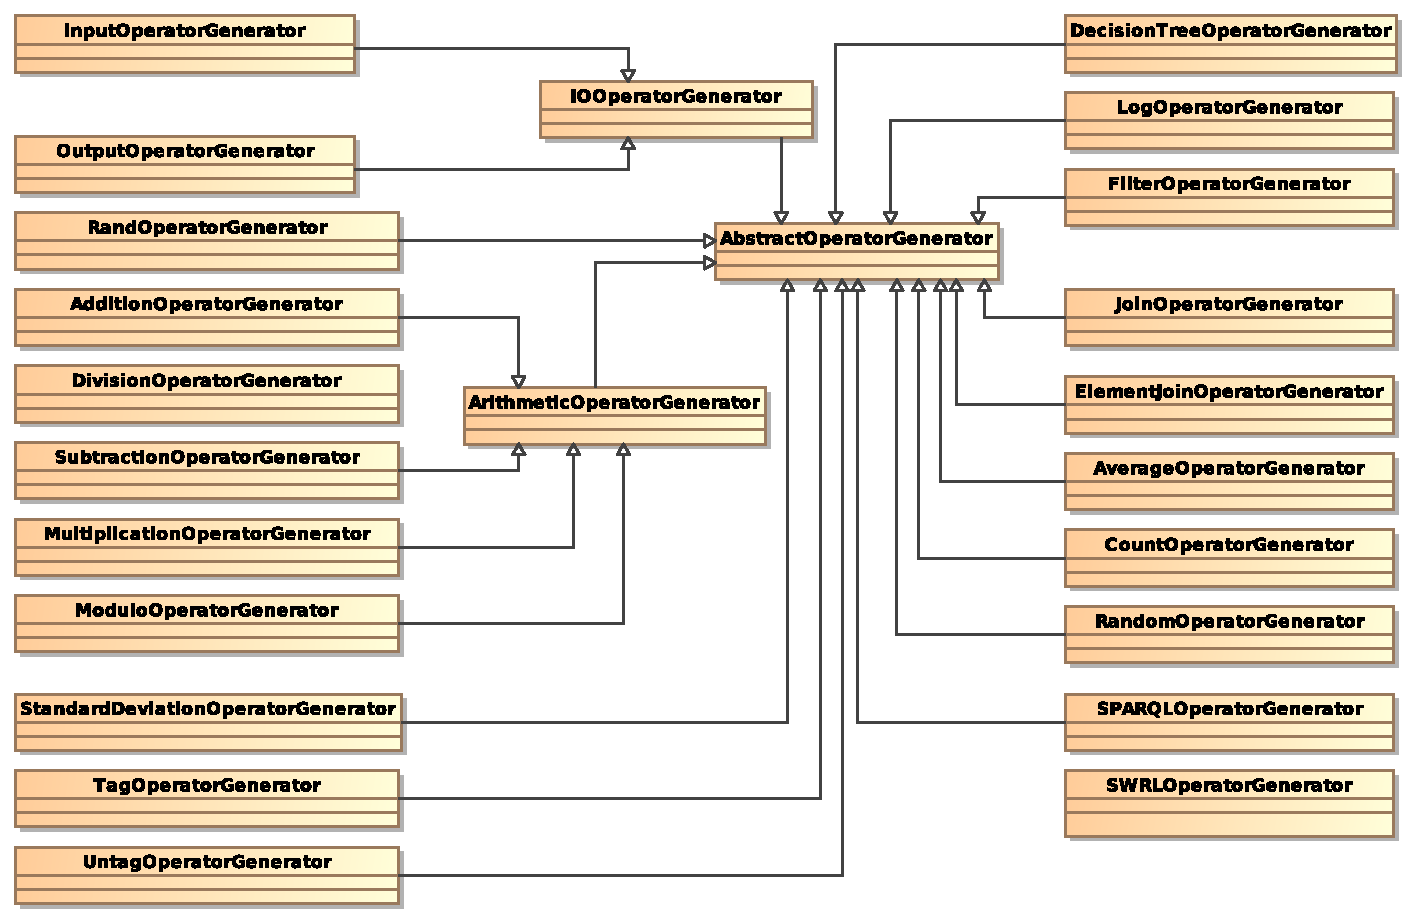
\includegraphics[width=1.0\textwidth]{figures/overview}
  \caption{\emph{Overview of classes which are used in code generation}}
  \label{fig:generator}
\end{figure}
Every operator of the query language is transformed into a set of LUA 
statements. The LUA script typically consists of statements for the 
initializiation of the framework, initialization and parameterization of 
operators, interconnecting operators, start and stop of operators. The class 
\texttt{AbstractOperatorGenerator} is depicted in figure 
\ref{fig:abstractoperatorgenerator} and provides abstract methods for the 
initialization (\texttt{initializeOperator()}), parameterization 
(\texttt{setOperatorProperties()}) and interconnection 
(\texttt{setOperatorConnection()}) of operators. Each operator generalizes from
\begin{figure}[htpb]
  \centering
  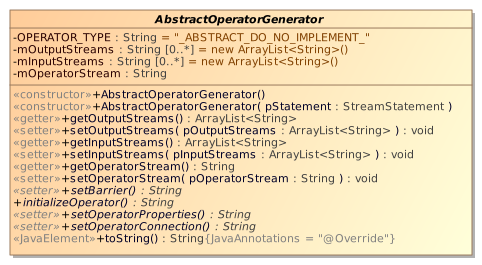
\includegraphics[width=0.7\textwidth]{figures/AbstractOperatorGenerator}
  \caption{\emph{UML class diagram of \texttt{AbstractOperatorGenerator}}}
  \label{fig:abstractoperatorgenerator}
\end{figure}
class \texttt{AbstractOperatorGenerator} and overwrites the abstract methods.

\subsubsection{Arithmetic Operators}
Supported arithmetic operators are \texttt{add} 
(\texttt{AdditionOperatorGenerator}), \texttt{sub} 
(\texttt{Subtraction\-OperatorGenerator}), \texttt{mult} 
(\texttt{MultiplicationOperatorGenerator}), \texttt{div} 
(\texttt{DivisionOperator\-Generator}) and \texttt{mod} 
(\texttt{ModuloOperatorGenerator}). Each operator inherits from class 
\texttt{Arithm\-eticperatorGenerator} which itself inherits from class
\texttt{AbstractOperatorGenerator}. Arithmetic operators are transformed to a
operator of type \texttt{Math}. The type of the arithmetic operation is set
as an attribute in LUA.

\begin{figure}[htpb]
  \centering
  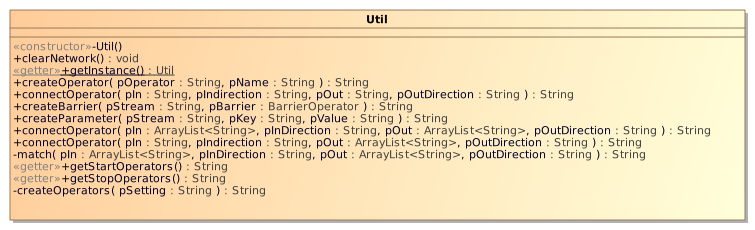
\includegraphics[width=0.9\textwidth]{figures/Util}
  \caption{\emph{UML class diagram of \texttt{Util}}}
  \label{fig:util}
\end{figure}

\subsubsection{Analysis Operators}
Analysis operatores are \texttt{avg} (\texttt{AverageOperatorGenerator}), 
\texttt{std} (\texttt{StandardDeviationOper\-atorGenerator}) and \texttt{count}
(\texttt{CountOperatorGenerator}).

\subsubsection{Structural Operators}

\subsubsection{Knowledge Operators}

\subsubsection{System Operators}
System operators are \texttt{in} (\texttt{InputOperatorGenerator}), 
\texttt{out} (\texttt{OutputOperatorGenerator}) and \texttt{log} 
(\texttt{LogOperatorGenerator}). The generators for the \texttt{in} and 
\texttt{out} operator are inheriting from a class \texttt{IOOperatorGenerator}.
The class transforms internationalized resource identifiers (IRI) to the 
corresponding LUA code. 

\section{Implementation}
\subsection{Introduction}
In a previous version of the query language, code was generated for a DSM system
specified in \cite{285:Fischer2010}. While the introduced system had its 
limitations, extensions for this system were defined in \cite{297:Frey2010}. In 
particular, this included a XML schema for the code generator, operators in the 
framework and a message format for the DSM framework. This work provides a code 
generator for LUA which forms the foundation for the rewritten DSM framework for 
the DataStreamMiner project. It is a complete rewrite of the code generator of 
previous versions of the query language.

The remainder of this section is organized as follows. First, building blocks of 
the query language such as streams, barriers and operators and their 
corresponding LUA counterpart are presented. Second, deprecated features of the 
query language are discussed followed by the integration of knowledge 
representations into the query language. The section concludes with a short
summary.
\begin{center}
  \begin{tabular}{|l|l|l|l|}
  \hline 
  \textbf{Operator Flow} &  \textbf{Operator LUA} &  \textbf{Comment} \\
  \hline 
  \hline 
  \texttt{avg} & IntAvg, \textit{FloatAvg} & computes the average value \\
  \hline 
  \texttt{count} & MessageCounter & counts a element in a stream \\
  \hline 
  \texttt{std} & \textit{StandardDeviation} & computes standard deviation of a element \\
  \hline 
  \texttt{add} & \textit{Math} & addition operation \\
  \hline 
  \texttt{sub} & \textit{Math} & subtraction operation \\
  \hline 
  \texttt{mult} & \textit{Math} & multiplication operation \\
  \hline 
  \texttt{div} & \textit{Math} & division operation \\
  \hline 
  \texttt{mod} & \textit{Math} & modulo operation \\
  \hline 
  \texttt{join} & Merge & joins multiple operators \\
  \hline 
  \texttt{ejoin} & \textit{ElementMerge} & adds elements to the stream \\
  \hline
  \texttt{split} & \textit{Split} & duplicates a stream \\
  \hline
  \texttt{filter} & \textit{Filter} & filter a stream after a multiple criterias \\
  \hline
  \texttt{tag} & \textit{Tag} & map elements stream/ontology \\
  \hline   
  \texttt{untag} & \textit{Untag} & map elements ontology/stream \\
  \hline 
  \texttt{swrl} &  \textit{SWRL} & operator for specification of SWRL rules \\
  \hline
  \texttt{dtree} & DecisionTree & decision tree \\
  \hline  
  \texttt{sparql} & Tag (Sparql) & specifies sparql queries \\
  \hline 
  \texttt{in} & CacheIn & input operator \\
  \hline
  \texttt{out} & CacheOut & output operator \\
  \hline
  \texttt{rand} & RandomInts & generates random integer values \\
  \hline
  - & PrintOnScreen & prints data on screen \\
  \hline  
  - & SeparateOddEven & operator for modulo two \\
  \hline  
  - & NumberGenerator & operator which generates numbers \\
  \hline  
  \texttt{log} & Log & log operator \\
  \hline
  \end{tabular}
  \captionof{table}{\emph{Comparision of operators in query language and framework}}
  \label{tab:overview}
\end{center}

\subsection{Language}
A comparison of operators in the query language and the corresponding operators 
in LUA is depicted in table \ref{tab:overview}. Operators set in italic are not 
implemented in the DataStreamMiner framework, but will be generated by the 
generator of the query language. For a full description of the operators of the
query language please be referred to \cite{297:Frey2010}. However, important 
changes to the design and behavior of operators is described in the 
corresponding sections.

\subsubsection{Streams}
While streams are the main entities of the query language, the DSM framework 
itself focuses on operators and the interconnection between them. Thus, streams
are set as parameters of an operator where a additional string denotes if it is 
a input or a output stream. Listing \ref{lst:stream} depicts an example where 
two streams \texttt{one} and \texttt{two} are connected to the input and output 
of an operator.
\begin{lstlisting}[language=Lua, caption={\emph{Example of Streams in LUA}},label={lst:stream}]
-- the strings represent the direction
fm:connect_operators(two, "out", one, "in");
\end{lstlisting}
The query language supports multiple streams as a return type, whereas the LUA
interface of the DSM framework only supports multiple streams for operators in
special cases. Hence, the generator of the query language transforms if required
multiple streams into several \texttt{split} operations where streams are 
copied.

\subsubsection{Barriers}
The query language introduced two types of barrier mechanisms 
\cite{297:Frey2010}. The first barrier mechanism provides a sliding window over
a stream of data, whereas the sliding window can be specified in terms of time
(seconds, minutes or hours) or elements. The second barrier mechanism is a 
marker mechanism which provides a special element in a data stream. Elements 
in a stream are processed while a marker passes the operator. For further 
information about the marker barrier mechanism please be referred to 
\cite{297:Frey2010}. Since the DSM framework does not support markers, the 
feature was disabled and might be included in future versions of the language 
and the DSM framework. Listing \ref{lst:exbaflw} shows an example for a barrier
in the average operator \texttt{avg} of the query language.
\begin{lstlisting}[language=Flow, caption={\emph{Example of Barrier Mechanism in Flow}},label={lst:exbaflw}]
// operation computes the average value of an element over the last 10 hours
a = avg(r.element, r[last 10 hrs]);
\end{lstlisting}
The barrier is transformed into the LUA construct depicted in listing 
\ref{lst:exbalua}. The barrier mechanism is transformed into a 
\texttt{set\_parameter()} operation of the operator. The first parameter in line
1 denotes the step size of the sliding window whereas the time is set in 
miliseconds. The last parameter in line 2 sets the type of the sliding window,
here it is \texttt{time}. Another option for the window type is 
\texttt{elements}. At present the \texttt{time} option only supports seconds,
minutes and hours. 
\begin{lstlisting}[language=Lua, caption={\emph{Example of Barrier Mechanism in LUA}},label={lst:exbalua}]
-- step_size_num denotes the step size, window_type the type of the window
a:set_parameter("step_size_num", "36000000");
a:set_parameter("window_type", "time");
\end{lstlisting}

\subsubsection{Operators}
The following section presents examples for operators written in the query 
language and the corresponding  transformation into LUA artifacts. Every 
operator is initialized by a \texttt{create\_operator\_of\_type}() operation. 
Paramters of each operator are set with a \texttt{set\_param\-eter()} operation 
which consists of a key/value structure. The first argument of the operation
denotes the key, the second argument the value of the key. Typically, input and
output streams of different operators are connected by the 
\texttt{connect\_operators()} operation. Parameters of the operation are the 
input and output streams and a string value which denotes the direction of the 
stream. 
\begin{lstlisting}[language=Flow, caption={\emph{Examples of Analysis Operators in Flow}},label={lst:exanflw}]
// Operation: Computes the average of an element 'element' in a stream r over the last 10 hours
a = avg(r.element, r[last 10 hrs]);
// Operation: Computes the standard deviation of an element 'element' in a stream s over the last 20 elements
b = std(s.element, s[last 20 elements]);
// Operation: Counts the occurrence of element 'element' in a stream t in the last 10 minutes
c = count(t.element, t[last 10 min]);
\end{lstlisting}
Analysis operators are average (\texttt{avg}), standard deviation (\texttt{std})
and count (\texttt{count}). Each operator has a parameter which denotes the 
element in a stream while the second parameter defines the sliding window over
the stream. Listing \ref{lst:exanflw} depicts examples for the analysis 
operators. The initialization of the streams is omitted. The operators 
specified in the previous listing are transformed in the corresponding LUA 
artifacts which are depicted in listing \ref{lst:exanlua}. Each operator is 
identified by a name which corresponds to the output stream of the operator. 
The first argument in the initialization of the operator identifies the output
stream of the operator, the second argument specifies the type of the operator. 
\begin{lstlisting}[language=Lua, caption={\emph{Examples of Analysis Operators in LUA}},label={lst:exanlua}]
-- average operator
a = fm:create_operator_of_type("a", "IntAvg");
a:set_parameter("step_size_num", "36000000");
a:set_parameter("window_type", "time");
a:set_parameter("element", "element");
fm:connect_operators(a, "out", r, "in");

-- standard deviation operator
b = fm:create_operator_of_type("b", "StandardDeviation");
b:set_parameter("step_size_num", "20");
b:set_parameter("window_type", "elements");
b:set_parameter("element", "element");
fm:connect_operators(b, "out", s, "in");

-- count operator
c = fm:create_operator_of_type("c", "MessageCounter");
c:set_parameter("step_size_num", "600000");
c:set_parameter("window_type", "time");
c:set_parameter("element", "element");
fm:connect_operators(c, "out", t, "in");
\end{lstlisting}
Arithmetic operators are addition (\texttt{add}), subtraction 
(\texttt{sub}), multiplication (\texttt{mult}), division (\texttt{div}) and
modulo (\texttt{mod}). Parameter of each arithmetic operator is an element in
a stream which represents the left operand of the arithmetic operation and
a right operand which can be a number, variable or another element in a stream. 
The result of each arithmetic operation is a value which is saved in a output
stream. Listing \ref{lst:exarflw} depicts an example for each arithmetic 
operator, whereas listing \ref{lst:exarflw} presents the arithmetic operators 
transformed into LUA artifacts.
\begin{lstlisting}[language=Flow, caption={\emph{Examples of Arithmetic Operators in Flow}},label={lst:exarflw}]
// Operation: d = u.element + 2
d = add(u.element, 2);
// Operation: e = v.element - o
e = sub(v.element, o);
// Operation: f = w.element * x.element
f = mult(w.element, x.element);
// Operation: g = y.element / 3
g = div(y.element, 3);
// Operation: h = a.element % z.element
h = mod(a.element, z.element); 
\end{lstlisting}
Bla
\begin{lstlisting}[language=LUA, caption={\emph{Examples of Arithmetic Operators in LUA}},label={lst:exanlua}]
-- Add
d = fm:create_operator_of_type("d", "Math");
d:set_parameter("operationType", "add");
d:set_parameter("literal", "2");
fm:connect_operators(d, "out", u, "in");
-- Sub
e = fm:create_operator_of_type("e", "Math");
e:set_parameter("operationType", "sub");
e:set_parameter("literal", "42");
fm:connect_operators(e, "out", v, "in");
-- Mult
f = fm:create_operator_of_type("f", "Math");
f:set_parameter("operationType", "mult");
f:set_parameter("stream", "x");
f:set_parameter("element", "element");
fm:connect_operators(f, "out", w, "in0");
fm:connect_operators(f, "out", x, "in1");
-- Div
g = fm:create_operator_of_type("g", "Math");
g:set_parameter("operationType", "div");
g:set_parameter("literal", "3");
fm:connect_operators(g, "out", y, "in");
-- Mod
h = fm:create_operator_of_type("h", "Math");
h:set_parameter("operationType", "mod");
h:set_parameter("stream", "z");
h:set_parameter("element", "element");
fm:connect_operators(h, "out", a, "in0");
fm:connect_operators(h, "out", z, "in1");
\end{lstlisting}
Structural operators are \texttt{join}, \texttt{ejoin} and \texttt{split}. The
following listing \ref{lst:exstructflw} depicts an example for each operation.
\begin{lstlisting}[language=Flow, caption={\emph{Examples of Structural Operators}},label={lst:exstructflw}]
// merges the two streams a and b
c = join(a, b);
// adds two elements to a stream b
d = ejoin(newElement, a.element, b);	
// filters stream on the stated condition
e = filter(d.element > 2, d);
\end{lstlisting}
The transformation of the previously presented operators is depicted in listing
\ref{lst:exstructlua}. The \texttt{join} operation specifies two input streams
and one output stream in line three and four. At present, the \texttt{ejoin} 
operator is not supported by the DSM framework. Parameters of the operator are
variables with an assigned value or elements of different streams, which are 
transformed into a set of assignments where the name and type of the element
is set by a \texttt{set\_parameter()} operation. The \texttt{filter} operator
allows to filter a stream by specifying boolean expressions which have to hold
true for a stream. Since no operator for boolean expressions is specified in the
LUA interface of the DSM framework, the expressions are compiled into a set of 
\texttt{set\_parameter()} operations where a expression is transformed to a 
textual representation of each aspect of an expression. This includes type and 
value of an operand as well as the operator of the boolean expression. 
\begin{lstlisting}[language=Lua, caption={\emph{Generated LUA code of Structural Operators}},label={lst:exstructlua}]
-- merge (join) operator
c = fm:create_operator_of_type("c", "Merge");
fm:connect_operators(c, "out", a, "in0");
fm:connect_operators(c, "out", b, "in1");
-- element join operation 
d = fm:create_operator_of_type("d", "ElementMerge");
d:set_parameter("name", "newElement");
d:set_parameter("type", "number");
d:set_parameter("value", "2");
d:set_parameter("stream_name", "a");
d:set_parameter("stream_element", "element");
d:set_parameter("stream_element_type", "int");
fm:connect_operators(d, "out", a, "in0");
fm:connect_operators(d, "out", b, "in1");
-- filter operation 
e = fm:create_operator_of_type("e", "Filter");
e:set_parameter("type", ">");
e:set_parameter("operand", "right");
e:set_parameter("datatype", "number");
e:set_parameter("value", "2");
e:set_parameter("operand", "left");
e:set_parameter("stream", "d");
e:set_parameter("element", "element");
fm:connect_operators(e, "out", d, "in");
\end{lstlisting}
System operatores are the input (\texttt{in}), output (\texttt{out}) and log
(\texttt{log}) operator. The input and ouput operators require a single 
internationalized resource identifier (IRI) or a list of IRIs, a address and a 
port. In addition, the output operator requires a input stream. The log operator
requires a location, a format and a input stream. Examples for the system 
operators are shown in listing \ref{lst:exsysflw}.
\begin{lstlisting}[language=Flow, caption={\emph{Examples of System Operators}},label={lst:exsysflw}]

// The location is a file called 'generated3.txt', the format is the file 'aal', input stream is 'dt'
logIn = log("generated3.txt", "aal", dt);
\end{lstlisting}

\begin{lstlisting}[language=Lua, caption={\emph{Generated LUA code of System Operators}},label={lst:exanlua}]
-- input/cachein operator
cacheIn = fm:create_operator_of_type("cacheIn", "CacheIn");
cacheIn:set_parameter("list_iris", "http://www.anothertest.de ");
cacheIn:set_parameter("connector_socket_address", "localhost");
cacheIn:set_parameter("connector_socket_port", "9595");
-- log operator
logIn = fm:create_operator_of_type("logIn", "Log");
logIn:set_parameter("log_file_location", "generated3.txt");
logIn:set_parameter("log_format", "aal");
fm:connect_operators(logIn, "out", dt, "in");
\end{lstlisting}

\subsection{Deprecated Features of the Query Language}
Operators and language features which were part of previous version of the query
language are denoted in table \ref{tab:deprecated}. The expressivness of a query
language is limited to the system on which the language is executed.

The transformation of procedural statements to a data stream mining system
has its limitations. Typically, such a system can be intepreted as a acyclic 
directed graph, where edges can be intepreted as streams and vertices as 
operators. Control structures such as loops violate the acyclic property of a 
acyclic directed graph. Conditional structurs such as 
if/else or switch statements can be expressed by means of the \texttt{filter}
operator and therefore are syntactic sugar. 
\begin{center}
  \begin{tabular}{|l|l|l|}
  \hline
  \textbf{Feature} & \textbf{Type} & \textbf{Comment} \\
  \hline
  \hline
  \texttt{map} & Operator & Operator for projections \\
  \hline
  marker & Operator & Mechanism for creating flexible barriers \\
  \hline
  \texttt{match} & Operator & Operator which compared two streams depending on a expression \\
  \hline
  \texttt{dif} & Operator & Operator for creating differences in sets (set theory) \\
  \hline
  \texttt{sdif} & Operator & Operator for creating symmetric differences in sets (set theory) \\
  \hline
  loops & Feature & Loop statements such as while  \\
  \hline
  conditions & Feature & Conditional statements such as if/else or switch/case \\
  \hline
  functions & Feature & Procedural functions for the map operator \\
  \hline
  \end{tabular}
  \captionof{table}{\emph{Deprecated features of the query language}}
  \label{tab:deprecated}
\end{center}

\subsection{Integration of Meta-models}
Xtext allows to reference instances of metamodels within a DSL. In order to use 
this mechanism several steps are required. The integration of OWL is used as an
example for the illustration of the integration process. Several steps are 
required in order to integrate a external metamodel into a Xtext DSL. First, the
metamodel must be referenced in the grammar of the language which is depicted in
listing \ref{lst:import}. In order to reference elements of the metamodel a 
unique identifier is assigned, here \texttt{owl}.
\begin{lstlisting}[language=Xtext, caption={\emph{Integration of the OWL ecore model into a grammar}},label={lst:import}]
import "platform:/resource/de.hs_rm.cs.vs.dsm.flow/model/owl.ecore"
   as owl
\end{lstlisting}
Second, the metamodel needs to be referecend in the MWE2 workflow of the main 
language plug-in. Listing \ref{lst:importmwe} shows how to register the
genmodel of the OWL metamodel in the MWE2 workflow definition of the query 
language.
\begin{lstlisting}[language=MWE2, caption={\emph{Integration of the OWL ecore model into a MWE2 workflow}},label={lst:importmwe}]
Workflow {
  bean = StandaloneSetup {
  ...
  platformUri = "${runtimeProject}/.."
    registerGenModelFile = "platform:/resource/de.hs_rm.cs.vs.dsm.flow/model/owl.genmodel"
\end{lstlisting}

\subsection{Summary}

\section{Summary}
The goal of this work was to provide a generator for the LUA interface of the
DSM framework. Future improvements and new research directions described in  
\cite{297:Frey2010} remain still open. This includes among others the definition
of new operators, the integration of knowledge tools in the RCP application, ...

The Xtext language toolkit provides mechanisms for the creation of DSLs
and DSL workbenches. This includes among others content assists, template 
proposals and quick fixes. Future developments of the query language and the 
language workbench might provide these features. However, the 
toolkit has its limitations.


\addcontentsline{toc}{section}{Literature}
\bibliographystyle{alphadin}
\bibliography{doc}

\end{document}
